\chapter{Prova de Conceito: \textit{Bot} para Interação Educacional}
\label{cap:prova}

% Usar o graphicspath para buscar figuras no subdiretório figuras
\graphicspath{\currfiledir/figuras/}

Este capítulo apresenta a prova de conceito do \textit{bot} educacional
desenvolvido para este trabalho, detalhando sua implementação técnica e a
metodologia de avaliação experimental proposta. O \textit{dashboard} contém
elementos que são a representação gráfica do \textit{bot}, permitindo ao
professor gerenciar as interações conforme estabelecido no Capítulo
\ref{cap:revisao}.

O Capítulo está organizado da seguinte forma: a Seção \ref{sec:contexto}
contextualiza a interação professor-aluno em ambientes remotos, como
estabelecido no Capítulo \ref{cap:revisao}, e como o \textit{bot} transforma
este paradigma, a Seção \ref{sec:implementacao} detalha os aspectos técnicos da
implementação, incluindo a arquitetura do sistema e as tecnologias utilizadas, a
Seção \ref{sec:funcionalidades} apresenta as funcionalidades implementadas no
\textit{bot} e no \textit{dashboard}, a Seção \ref{sec:metodologia} descreve a
metodologia de avaliação experimental proposta, e finalmente, a Seção
\ref{sec:resultados} apresenta os resultados ilustrativos obtidos na validação
do sistema.

\section{Contexto da Interação Professor-Aluno em Ambientes Remotos}
\label{sec:contexto}

Como visto na Seção \ref{sec:motivacao}, em uma aula remota tradicional é
frequentemente observada uma comunicação unidirecional, onde o professor
apresenta o conteúdo enquanto os alunos assumem postura predominantemente
passiva.

O \textit{bot} proposto busca transformar este paradigma ao introduzir um
mediador digital que facilita:

\begin{enumerate}
\item \textbf{Trocas síncronas durante a exposição de conteúdo}: Permitindo
reações e dúvidas sem interromper o fluxo da aula
\item \textbf{Anonimato seletivo para alunos}: Reduzindo a inibição de
participação
\item \textbf{Coleta sistemática de dados de interação}: Possibilitando ajustes
em tempo real na condução da aula
\item \textbf{Automação de tarefas repetitivas}: Liberando o professor para
focar em aspectos pedagógicos mais relevantes
\end{enumerate}

Entendemos que estas características são fundamentais para aproximar o ambiente
virtual das dinâmicas interativas observadas em salas de aula presenciais onde
metodologias ativas são aplicadas com sucesso.

\section{Implementação Técnica}
\label{sec:implementacao}

A implementação técnica do sistema educacional segue uma arquitetura dual
composta pelo \textit{bot} Discord e pelo \textit{dashboard} do professor,
conforme conceitualmente apresentado na Seção \ref{subsec:dashboards}. Esta
arquitetura garante a separação entre o canal de comando (exclusivo do
professor) e o canal de interação (compartilhado entre todos os participantes).

Esta seção está organizada da seguinte forma: a Seção
\ref{subsec:arquitetura-bot} detalha a arquitetura modular do \textit{bot}
desenvolvido em C utilizando a biblioteca Concord, a Seção
\ref{subsec:dashboard-impl} apresenta a implementação do \textit{dashboard} web
e sua comunicação com o \textit{bot}, e a Seção \ref{subsec:integracao-tecnica}
aborda os aspectos de integração técnica e conformidade com os componentes
essenciais de um \textit{bot} educacional estabelecidos no referencial teórico.

\subsection{Arquitetura do \textit{Bot}}
\label{subsec:arquitetura-bot}

O \textit{bot} foi desenvolvido utilizando a biblioteca Concord em C, como visto
na Seção \ref{sec:ferramentas}. A implementação seguiu uma arquitetura modular
organizada em quatro componentes principais, (1) módulos de publicação, (2)
interação, (3) análise e (4) persistência. Estes módulos foram escolhidos para
atender aos objetivos pedagógicos e técnicos estabelecidos no Capítulo
\ref{cap:revisao}:

\begin{itemize}
\item \textbf{Módulo de Publicação}: Responsável por processar comandos do
professor vindos do \textit{dashboard} e transformá-los em conteúdo formatado
nos canais apropriados do Discord. Este módulo implementa recursos de formatação
para código, imagens e outros materiais didáticos.
\item \textbf{Módulo de Interação}: Gerencia as reações e comandos dos alunos,
incluindo o processamento de comandos \textit{slash}, reações com emojis e
mensagens diretas. Este componente implementa o princípio de comunicação
multidirecional discutido na Seção \ref{subsec:principios}.
\item \textbf{Módulo de Análise}: Coleta e processa em tempo real as interações
para gerar métricas de engajamento, barômetros de compreensão e outros
indicadores pedagógicos relevantes. Os resultados são transmitidos ao
\textit{dashboard} do professor para visualização.
\item \textbf{Módulo de Persistência}: Armazena dados estruturados sobre a
sessão para análise posterior, possibilitando a geração de relatórios detalhados
e o acompanhamento longitudinal do progresso dos alunos ao longo de múltiplas
aulas.
\end{itemize}

\begin{figure}[H] \centering
\centering
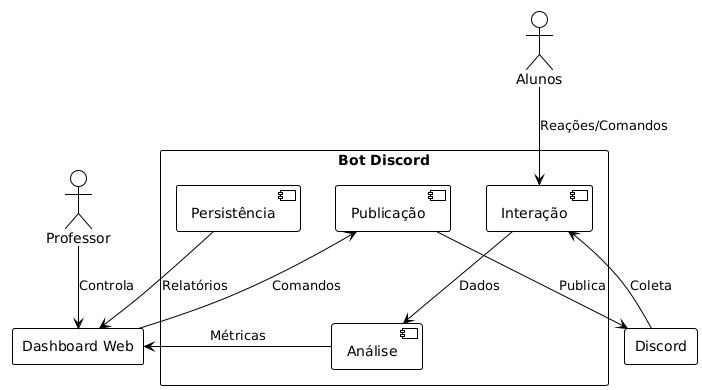
\includegraphics[width=16cm]{arquitetura-bot.png}
\caption{Arquitetura do \textit{bot} educacional, mostrando os principais
módulos e a comunicação com o \textit{dashboard} do professor.}
\label{fig:arquitetura-bot}
\end{figure}

\subsection{Implementação do \textit{Dashboard}}
\label{subsec:dashboard-impl}

O \textit{dashboard} do professor foi implementado como uma aplicação web
utilizando tecnologias consolidadas de frontend (JavaScript) e backend
(Node.js), comunicando-se com o \textit{bot} através de uma \textit{API REST}.
Esta separação arquitetural permite que o professor mantenha uma interface de
controle independente e privada, sem necessidade de interagir diretamente no
\textit{chat} público.

O sistema de comunicação entre \textit{dashboard} e \textit{bot} utiliza um
protocolo de mensagens baseado em \textit{WebSocket} para garantir atualizações
em tempo real e baixa latência, aspectos cruciais para o controle efetivo da
dinâmica da aula. Esta comunicação bidirecional permite:

\begin{enumerate}
\item Envio de comandos do professor para o \textit{bot} (publicação de
conteúdo, criação de atividades)
\item Transmissão de métricas e alertas do \textit{bot} para o
\textit{dashboard} (nível de engajamento, dúvidas anônimas)
\item Sincronização do estado da aula entre múltiplas sessões de navegador, caso
o professor precise alternar entre dispositivos
\end{enumerate}

\begin{figure}[H] \centering
\centering
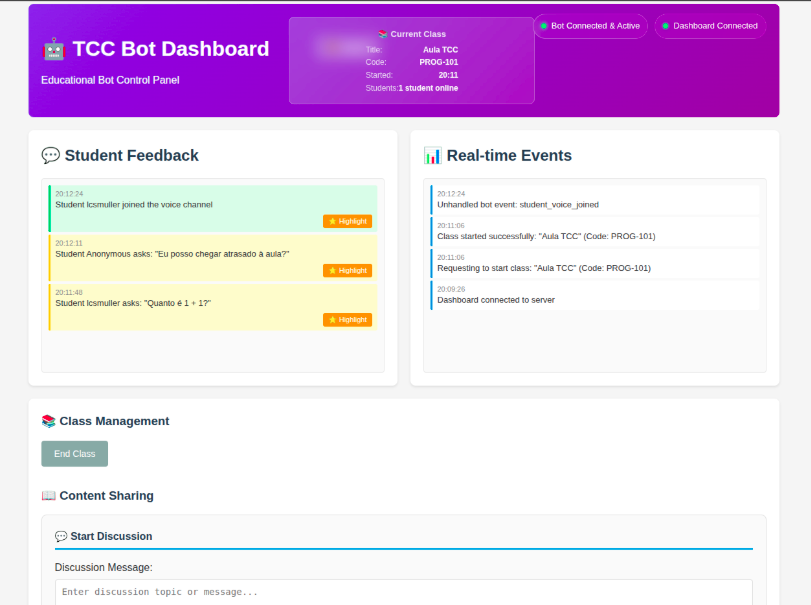
\includegraphics[width=16cm]{dashboard-preview.png}
\caption{Visão geral do \textit{dashboard} do professor, mostrando as principais
funcionalidades e a integração com o \textit{bot} educacional.}
\label{fig:dashboard-preview}
\end{figure}

\subsection{Integração Técnica}
\label{subsec:integracao-tecnica}

A integração com o Discord foi realizada através das \textit{APIs} fornecidas
pela biblioteca Concord.

A arquitetura implementa os cinco componentes essenciais de um \textit{bot}
educacional descritos na Seção \ref{sec:def-bots}: (1) interface do usuário
(canais do Discord), (2) compreensão de linguagem natural (processamento de
comandos), (3) gerenciador de diálogo (módulo de interação), (4) integração com
backend (\textit{dashboard} e sistemas de persistência) e (5) geração de
resposta (módulo de publicação).

Esta implementação atende diretamente ao objetivo de criar uma prova de conceito
funcional utilizando tecnologias adequadas ao contexto educacional, conforme
estabelecido na Seção \ref{sec:objetivos}.

O código-fonte completo da implementação, incluindo o \textit{bot} educacional 
e o \textit{dashboard} de controle pedagógico, está disponível no repositório 
público documentado no Apêndice \ref{appendix:repo}.

\section{Funcionalidades Implementadas}
\label{sec:funcionalidades}

Como visto na Seção \ref{sec:implementacao}, o sistema desenvolvido consiste em
dois componentes principais que trabalham de forma integrada: (1) o \textit{bot}
educacional que interage diretamente com os alunos no Discord e (2) o
\textit{dashboard} exclusivo para o professor que permite gerenciar essas
interações.

Esta seção está organizada da seguinte forma: a Seção
\ref{subsec:funcionalidades-bot} apresenta as funcionalidades implementadas no
\textit{bot} e no \textit{dashboard}, a Seção
\ref{subsec:funcionalidades-dashboard} detalha as funcionalidades do
\textit{dashboard} do professor, e a Seção \ref{subsec:comandos-implementados}
lista os comandos implementados e os cenários de uso.

\subsection{Funcionalidades do \textit{Bot} no Discord}
\label{subsec:funcionalidades-bot}

O \textit{bot} no ambiente Discord oferece as funcionalidades de (1) mecanismos
de \textit{feedback} rápido, (2) canal de dúvidas anônimas, (3) execução de
código e (4) atividades interativas:

\begin{enumerate}
\item \textbf{Mecanismos de \textit{feedback} rápido}: Permite que alunos
utilizem reações para indicar seu nível de compreensão (como ``entendi'', ``tenho
dúvida'', ``confuso''), criando um barômetro de compreensão em tempo real 
(Figuras \ref{fig:func-alunos-discussao} e \ref{fig:func-alunos-reacoes}).
\item \textbf{Canal de dúvidas anônimas}: Os alunos podem enviar dúvidas de
forma privada para o \textit{bot}, que as encaminha ao professor sem identificar
o remetente, reduzindo a inibição (Figuras \ref{fig:func-alunos-ask} a 
\ref{fig:func-alunos-ask-dashboard}).
\item \textbf{Execução de código}: Para disciplinas de programação, o
\textit{bot} permite a execução de snippets de código submetidos pelos alunos,
mostrando resultados em tempo real.
\item \textbf{Atividades interativas}: Disponibiliza \textit{quizzes}, enquetes
e desafios temporalizados, coletando e organizando as respostas dos alunos
automaticamente.
\end{enumerate}

\begin{figure}[H]
\centering
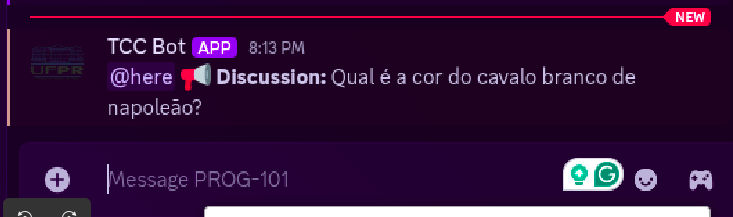
\includegraphics[width=0.8\textwidth]{func-alunos/iniciada-discussao.png}
\caption{Exemplo de discussão iniciada pelo professor, mostrando como o conteúdo é apresentado aos alunos no Discord.}
\label{fig:func-alunos-discussao}
\end{figure}

\begin{figure}[H]
\centering

\includegraphics[width=0.8\textwidth]{func-alunos/reacao-iniciada-discussao.png}
\caption{Reações dos alunos em uma discussão ativa, demonstrando o mecanismo de \textit{feedback} rápido através de emojis.}
\label{fig:func-alunos-reacoes}
\end{figure}

\begin{figure}[H]
\centering
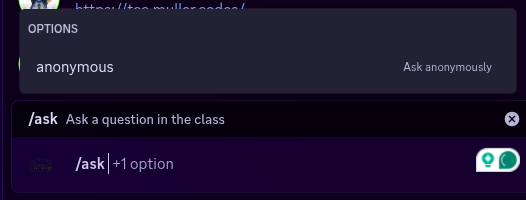
\includegraphics[width=0.8\textwidth]{func-alunos/comando-ask.png}
\caption{Comando \textbf{/ask} sendo utilizado por um aluno para enviar uma pergunta anônima ao professor.}
\label{fig:func-alunos-ask}
\end{figure}

\begin{figure}[H]
\centering
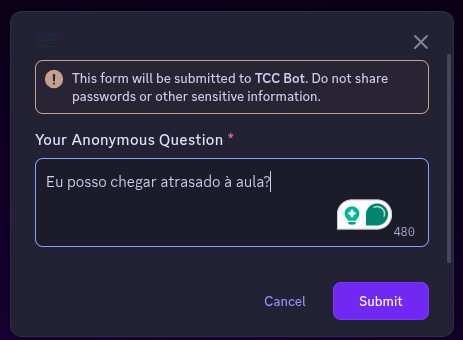
\includegraphics[width=0.8\textwidth]{func-alunos/comando-ask-modal.png}
\caption{Modal de texto do comando \textbf{/ask}, mostrando a interface para envio de perguntas com opção de anonimato.}
\label{fig:func-alunos-ask-modal}
\end{figure}

\begin{figure}[H]
\centering
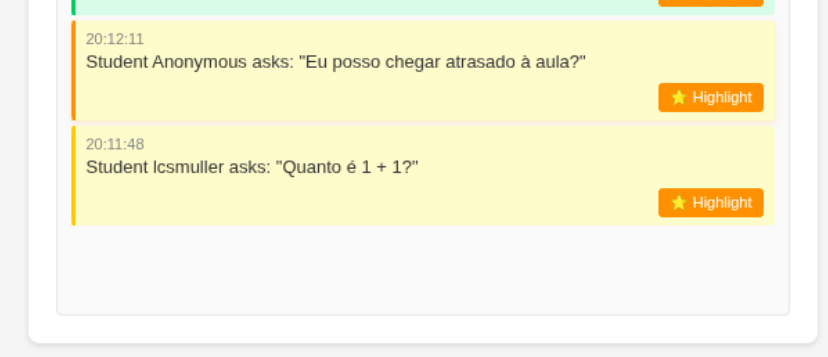
\includegraphics[width=0.8\textwidth]{func-alunos/comando-ask-visao-dashboard.png}
\caption{Visão do professor no dashboard ao receber uma pergunta anônima de um aluno através do comando \textbf{/ask}.}
\label{fig:func-alunos-ask-dashboard}
\end{figure}

\subsection{Funcionalidades do \textit{Dashboard} do Professor}
\label{subsec:funcionalidades-dashboard}

O \textit{dashboard}, como interface de controle pedagógico, implementa as
funcionalidades (1) sistema de alertas, (2) gerenciador de atividades e (3)
relatórios pós-aula:

\begin{enumerate}
\item \textbf{Sistema de alertas}: Notificações em tempo real sobre eventos
críticos da aula, incluindo alertas de conectividade com o bot, notificações de
entrada/saída de alunos no canal de voz, e indicadores visuais de problemas
técnicos. O sistema monitora continuamente o status da conexão e exibe alertas
imediatos quando há perda de comunicação com o \textit{bot} educacional
(Figura \ref{fig:func-prof-alertas}).
\item \textbf{Gerenciador de atividades}: Interface completa para criação,
lançamento e monitoramento de atividades interativas, incluindo discussões com
formatação automática, enquetes com opções dinâmicas (2-10 opções), snippets de
código com suporte a múltiplas linguagens, e controle de duração temporizada. O
sistema permite iniciar, pausar e finalizar atividades em tempo real, com
visualização simultânea de reações dos alunos e respostas agrupadas por tipo de
atividade (Figuras \ref{fig:func-prof-atividades-1}, \ref{fig:func-prof-atividades-2} 
e \ref{fig:func-prof-reacoes}).
\item \textbf{Relatórios pós-aula}: Geração automática de resumos detalhados ao
final da sessão, incluindo métricas de participação (número de estudantes
únicos, pico de participação, duração total da aula), histórico completo de
conteúdos ativos compartilhados com tempo de duração e estatísticas de
engajamento, registro de mensagens destacadas pelo professor durante a aula, e
timeline cronológica das respostas dos alunos vinculadas ao contexto do conteúdo
ativo (Figuras \ref{fig:func-prof-relatorios-1} e \ref{fig:func-prof-relatorios-2}).
\end{enumerate}

\begin{figure}[H]
\centering
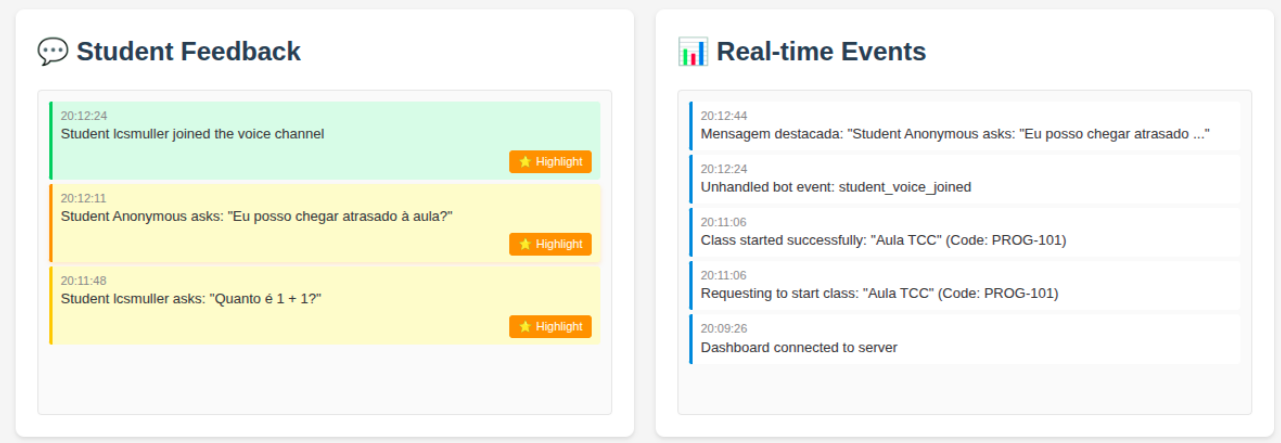
\includegraphics[width=0.8\textwidth]{func-professores/sistema-alertas.png}
\caption{Sistema de alertas do dashboard, mostrando notificações em tempo real sobre eventos críticos da aula.}
\label{fig:func-prof-alertas}
\end{figure}

\begin{figure}[H]
\centering
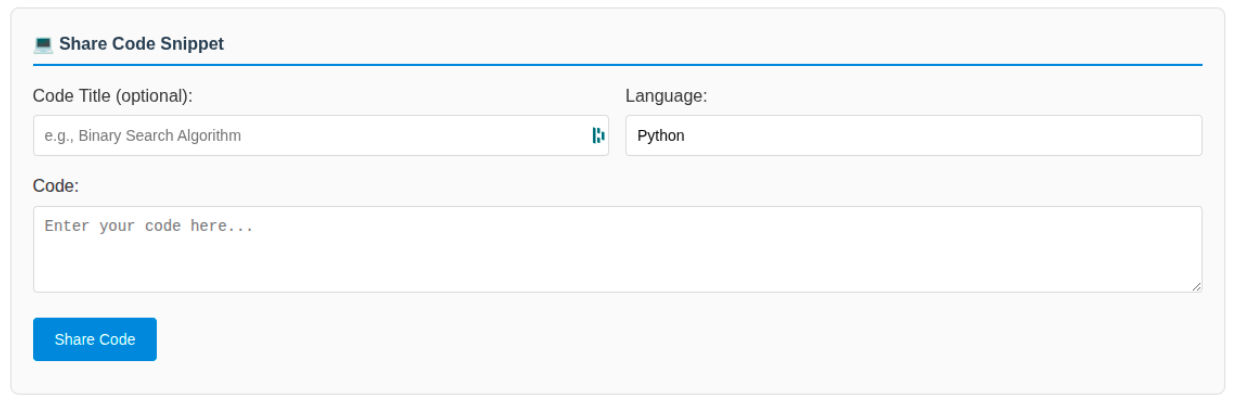
\includegraphics[width=0.8\textwidth]{func-professores/gerenciamento-atividades-parte1.png}
\caption{Interface do gerenciador de atividades - Parte 1: Criação e configuração de atividades interativas.}
\label{fig:func-prof-atividades-1}
\end{figure}

\begin{figure}[H]
\centering
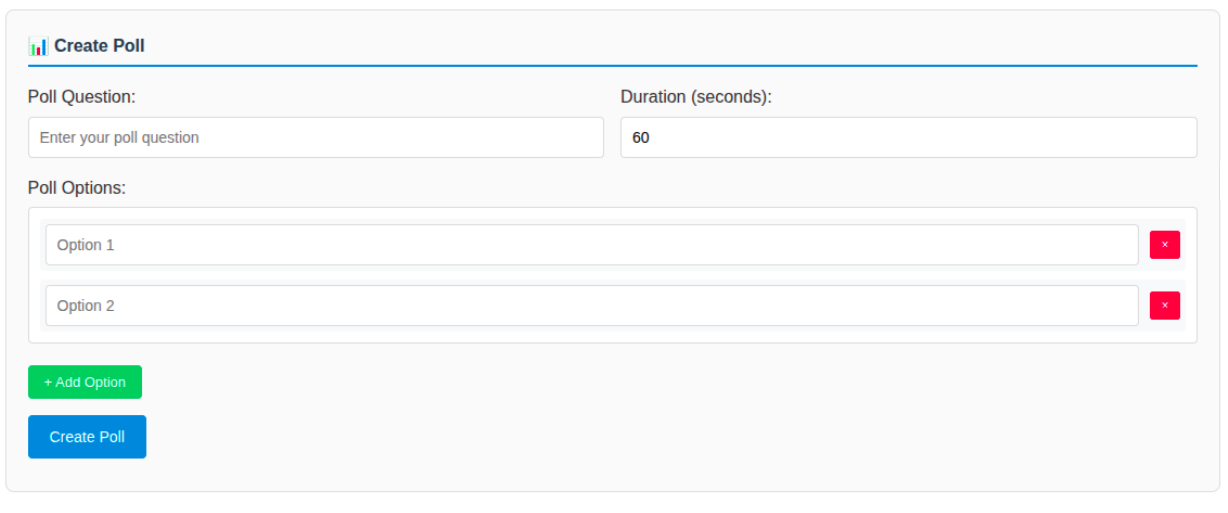
\includegraphics[width=0.8\textwidth]{func-professores/gerenciamento-atividades-parte2.png}
\caption{Interface do gerenciador de atividades - Parte 2: Monitoramento e controle de atividades em tempo real.}
\label{fig:func-prof-atividades-2}
\end{figure}

\begin{figure}[H]
\centering
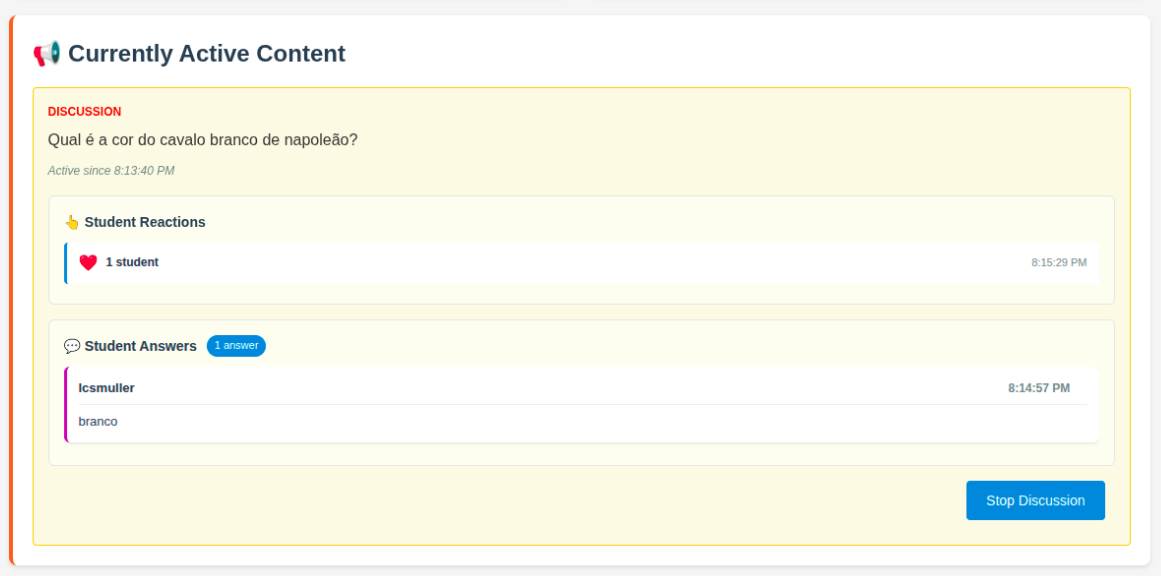
\includegraphics[width=0.8\textwidth]{func-professores/agregacao-reacao.png}
\caption{Agregação visual de reações dos alunos, permitindo ao professor visualizar o \textit{feedback} coletivo em tempo real.}
\label{fig:func-prof-reacoes}
\end{figure}

\begin{figure}[H]
\centering
\includegraphics[width=0.8\textwidth]{func-professores/relatórios-parte1.png}
\caption{Relatórios pós-aula - Parte 1: Métricas de participação e estatísticas gerais da sessão.}
\label{fig:func-prof-relatorios-1}
\end{figure}

\begin{figure}[H]
\centering
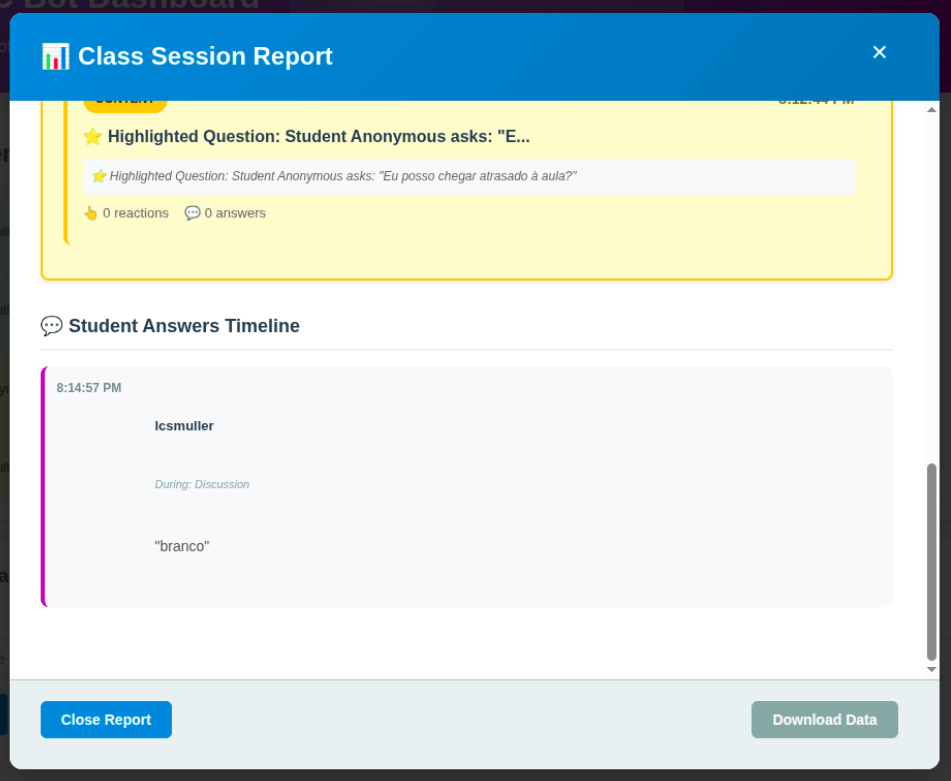
\includegraphics[width=0.8\textwidth]{func-professores/relatorios-parte2.png}
\caption{Relatórios pós-aula - Parte 2: Timeline cronológica das interações e detalhamento das atividades.}
\label{fig:func-prof-relatorios-2}
\end{figure}

A integração entre \textit{dashboard} e \textit{bot} visa criar um sistema coeso
que permite ao professor manter o controle pedagógico da aula enquanto facilita
interações dinâmicas com os alunos. O professor pode, por exemplo, identificar
rapidamente conceitos que geraram confusão através do \textit{dashboard} e
adaptar sua abordagem ou enviar explicações adicionais através do \textit{bot},
sem interromper o fluxo da aula.

As Figuras \ref{fig:func-alunos-discussao} a \ref{fig:func-alunos-ask-dashboard} 
ilustram o funcionamento das principais funcionalidades do \textit{bot} do ponto 
de vista dos alunos, enquanto as Figuras \ref{fig:func-prof-alertas} a 
\ref{fig:func-prof-relatorios-2} apresentam as interfaces do \textit{dashboard} 
utilizadas pelo professor para gerenciar e monitorar as atividades educacionais.

\subsection{Comandos Implementados e Cenários de Uso}
\label{subsec:comandos-implementados}

O sistema implementa um conjunto específico de comandos \textit{slash} no
Discord que permitem aos alunos interagir com o conteúdo da aula de forma
estruturada, os comandos criados são (1) \textbf{/help}, (2) \textbf{/ask
[anonymous]}, (3) \textbf{/answer [anonymous]} e (4) \textbf{/execute}:

\begin{enumerate}
\item \textbf{/help}: Exibe informações sobre os comandos disponíveis e como
utilizar o \textit{bot} educacional.
\item \textbf{/ask [anonymous]}: Permite enviar perguntas ao professor, com
opção de anonimato. Abre um modal de texto com limite de 512 caracteres.
\item \textbf{/answer [anonymous]}: Permite responder ao conteúdo ativo atual
(discussões, enquetes, exercícios), com opção de anonimato. Abre um modal de
texto com limite de 1024 caracteres.
\item \textbf{/execute}: Executa snippets de código compartilhados pelo
professor.
\end{enumerate}

Adicionalmente, o bot detecta automaticamente reações com emojis em mensagens de
conteúdo ativo, permitindo \textit{feedback} rápido através de símbolos como
``polegar para cima'' (entendi), ``ponto de interrogação'' (dúvida), ou ``rosto
confuso'' (confuso).

O \textit{dashboard} do professor suporta os cenários pedagógicos de (1)
discussões guiadas, (2) enquetes interativas, (3) compartilhamento de código e
(4) monitoramento de engajamento:

\begin{enumerate}
\item \textbf{Discussões guiadas}: Lançamento de tópicos de discussão com
acompanhamento das respostas dos alunos em tempo real.
\item \textbf{Enquetes interativas}: Criação de enquetes com 2-10 opções,
visualização das respostas e estatísticas de participação.
\item \textbf{Compartilhamento de código}: Envio de snippets de código com
sintaxe destacada para múltiplas linguagens de programação.
\item \textbf{Monitoramento de engajamento}: Visualização em tempo real de
reações, mensagens destacadas e participação dos alunos.
\end{enumerate}

A Figura \ref{fig:dashboard-bot} (Capítulo \ref{cap:revisao}) ilustra esta
relação integrada, onde o \textit{dashboard} atua como interface de comando
exclusiva do professor, enquanto o \textit{bot} serve como ponto de contato e
interação para todos os participantes.

\section{Metodologia de Avaliação}
\label{sec:metodologia}

A metodologia de avaliação para o \textit{bot} educacional consiste em uma
abordagem experimental com participantes reais assumindo os papéis de professor
e alunos em um ambiente de sala de aula simulado, conforme delineado na Seção
\ref{subsec:validacao-metodologia}. Esta abordagem permite avaliar a eficácia da
ferramenta em condições próximas ao uso real, combinando métricas quantitativas
e qualitativas.

Esta seção está organizada da seguinte forma: a Seção \ref{subsec:desenho}
apresenta o desenho experimental adotado, incluindo a estrutura das sessões e
características dos participantes, a Seção \ref{subsec:ambiente} descreve o
ambiente controlado utilizado e o perfil dos participantes, a Seção
\ref{subsec:coleta} detalha os mecanismos de coleta de dados empregados, e
finalmente, a Seção \ref{subsec:dimensoes-metricas} apresenta as dimensões de
avaliação e métricas utilizadas para mensurar a eficácia do sistema.

\subsection{Desenho Experimental}
\label{subsec:desenho}

O experimento foi estruturado com os seguintes parâmetros:

\begin{itemize}
\item \textbf{Participantes}: 10 usuários (8 da área da informática, 2 da área
de humanas), garantindo diversidade de perspectivas sobre tecnologia educacional
\item \textbf{Formato}: Experimentos individuais com cada participante,
permitindo avaliação personalizada das interações
\item \textbf{Estrutura das sessões}: 20 sessões experimentais no total, onde
cada participante atuou duas vezes - uma como professor (controlando o
\textit{dashboard}) e outra como aluno (interagindo via Discord)
\item \textbf{Duração}: Sessões de aproximadamente 30-45 minutos cada, tempo
suficiente para explorar as principais funcionalidades do sistema
\end{itemize}

\subsection{Ambiente e Participantes}
\label{subsec:ambiente}

O experimento foi conduzido em ambiente controlado que reproduziu condições de
ensino remoto:

\begin{itemize}
\item \textbf{Cenários pedagógicos}: Sessões simuladas abordando diferentes
tipos de conteúdo, incluindo aulas expositivas, discussões guiadas e atividades
práticas
\item \textbf{Equipamentos}: Participantes utilizaram seus próprios dispositivos
(computadores, tablets, smartphones), simulando condições reais de acesso
\item \textbf{Conectividade}: Teste realizado com diferentes condições de
conexão à internet
\item \textbf{Roles alternados}: Cada participante experienciou ambas as
perspectivas (professor e aluno), proporcionando visão abrangente do sistema
\end{itemize}

\subsection{Coleta de Dados}
\label{subsec:coleta}

Os dados foram coletados através de (1) questionários estruturados e (2)
comentários livres dos participantes:

\begin{enumerate}
\item \textbf{Questionários estruturados}: Aplicados imediatamente após cada
sessão experimental, medindo percepções sobre usabilidade, eficácia pedagógica e
aceitação da tecnologia.
\item \textbf{Comentários livres}: Espaço para feedback qualitativo aberto,
permitindo identificação de aspectos não cobertos pelas questões estruturadas
\end{enumerate}

\subsection{Dimensões de Avaliação e Métricas Utilizadas}
\label{subsec:dimensoes-metricas}

A avaliação foi estruturada em quatro dimensões principais, escolhidas de forma
exploratória para capturar diferentes aspectos da experiência com o \textit{bot}
educacional. É importante ressaltar que a seleção dessas dimensões foi realizada
de maneira arbitrária pelo autor, baseada em aspectos considerados relevantes
para a avaliação de ferramentas educacionais interativas. Para estudos futuros,
recomenda-se a utilização de frameworks de avaliação já consolidados na
literatura, como o Technology Acceptance Model (TAM) ou o Unified Theory of
Acceptance and Use of Technology (UTAUT), que oferecem metodologias mais
rigorosas e comparáveis.

As dimensões avaliadas e suas respectivas métricas são apresentadas a seguir:

\begin{table}[H]
\centering
\caption{Dimensões e métricas para avaliação da eficácia do \textit{bot}}
\label{tab:dimensoes-metricas}
\begin{tabular}{|p{3cm}|p{9cm}|}
\hline
\textbf{Dimensão} & \textbf{Métricas e Indicadores} \\
\hline
\textbf{Engajamento dos alunos} & Número e diversidade de interações, tempo de
resposta, participação voluntária em atividades, distribuição temporal das
interações \\
\hline
\textbf{Eficácia pedagógica} & Percepção de aprendizagem, clareza da comunicação,
suporte às metodologias ativas, mudanças na condução da aula, percepção de
compreensão do conteúdo, tempo dedicado a esclarecimentos \\
\hline
\textbf{Usabilidade da ferramenta} & Facilidade de uso, intuitividade da
interface, curva de aprendizado para professores e alunos, problemas técnicos,
satisfação com a interface \\
\hline
\textbf{Aceitação da tecnologia} & Disposição para adoção em contexto real,
percepção de utilidade, integração ao fluxo de trabalho pedagógico, comparação
com ferramentas tradicionais \\
\hline
\end{tabular}
\end{table}

Cada dimensão foi operacionalizada através de questões específicas no
questionário estruturado, permitindo uma avaliação multidimensional do sistema
desenvolvido. A escolha por uma abordagem exploratória se justifica pelo caráter
inicial desta pesquisa.

\section{Resultados Ilustrativos}
\label{sec:resultados}

Esta seção apresenta os resultados obtidos na avaliação do \textit{bot}
educacional, com base na metodologia descrita na Seção \ref{sec:metodologia}. Os
resultados são apresentados em duas partes: a Seção \ref{subsec:dados-quant}
apresenta a análise quantitativa dos dados coletados através dos questionários
aplicados aos participantes, e a Seção \ref{subsec:analise-qual} apresenta a
análise qualitativa dos comentários e feedbacks dos usuários.

\subsection{Dados Quantitativos}
\label{subsec:dados-quant}

A análise quantitativa dos questionários revelou resultados promissores em
múltiplas dimensões avaliadas. As respostas foram coletadas em escala de 1 a 5,
onde 1 representa ``muito insatisfatório'' e 5 representa ``muito
satisfatório''.

Esta seção está organizada da seguinte forma: a Seção
\ref{subsec:usabilidade-facilidade} apresenta os resultados sobre usabilidade e
facilidade de uso, a Seção \ref{subsec:eficacia-pedagogica} aborda a eficácia
pedagógica do \textit{bot}, a Seção \ref{subsec:funcionalidades-mais-utilizadas}
apresenta as funcionalidades mais utilizadas pelos participantes, a Seção
\ref{subsec:reduz-carga-comunicacao} analisa a redução de carga de trabalho do
professor e a facilitação da comunicação, e a Seção
\ref{subsec:aceitacao-adocao} discute a aceitação e adoção da tecnologia.

E se baseia na análise dos gráficos apresentados à seguir, que foram
extraídos dos questionários aplicados aos participantes, conforme descrito na
Seção \ref{subsec:coleta}:


\begin{figure}[H]
\centering
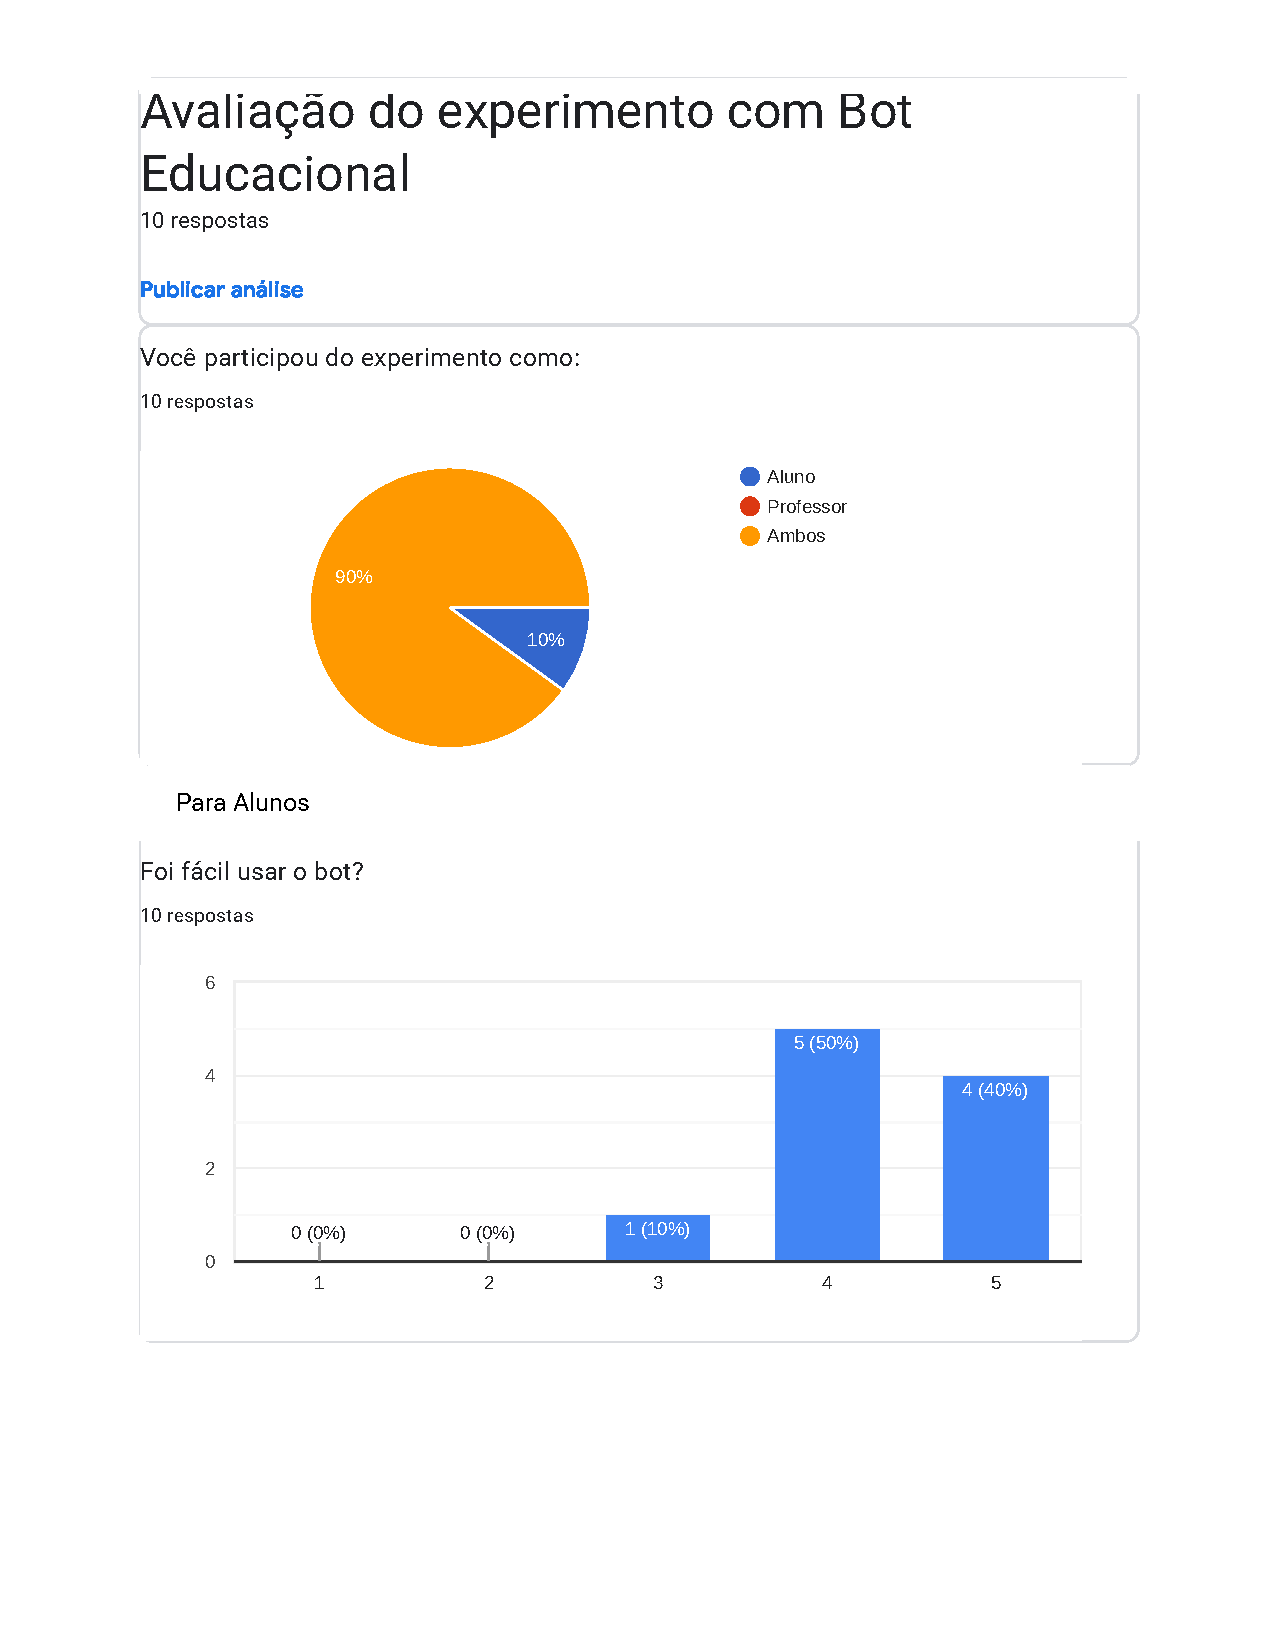
\includegraphics[
    page=1,
    trim={1cm 5cm 1cm 5.7cm},
    clip=true,
    width=0.8\textwidth
]{forms.pdf}
\caption{Distribuição das respostas sobre facilidade de uso do \textit{bot} e
dashboard. O gráfico superior mostra a distribuição dos papéis dos participantes
(aluno, professor, ambos), enquanto o gráfico inferior apresenta a avaliação da
facilidade de uso do \textit{bot}.}
\label{fig:usabilidade-bot}
\end{figure}

\begin{figure}[H]
\centering
\includegraphics[
    page=2,
    trim={1cm 9cm 1cm 1cm},
    clip=true,
    width=0.8\textwidth
]{forms.pdf}
\caption{Avaliação da facilidade de uso do dashboard do professor. O gráfico
superior mostra a percepção sobre como o \textit{bot} ajudou na compreensão do
conteúdo, enquanto o gráfico inferior apresenta a avaliação da facilidade de uso
do dashboard.}
\label{fig:usabilidade-dashboard}
\end{figure}

\begin{figure}[H]
\centering
\includegraphics[
    page=3,
    trim={1cm 1cm 1cm 1cm},
    clip=true,
    width=0.8\textwidth
]{forms.pdf}
\caption{Avaliação da eficácia pedagógica. O gráfico superior mostra se o
dashboard ajudou no monitoramento das atividades, o gráfico do meio apresenta a
experiência prévia dos participantes com EAD, e o gráfico inferior indica a
satisfação com EAD antes do experimento.}
\label{fig:eficacia-pedagogica}
\end{figure}

\begin{figure}[H]
\centering
\includegraphics[
    page=4,
    trim={1cm 1cm 1cm 1cm},
    clip=true,
    width=0.8\textwidth
]{forms.pdf}
\caption{Funcionalidades utilizadas e impacto na carga de trabalho e
interatividade. O gráfico superior mostra as funcionalidades mais utilizadas
durante o experimento, o gráfico do meio apresenta a percepção sobre redução da
carga na aula, e o gráfico inferior indica como o \textit{bot} tornou a aula
mais interativa.}
\label{fig:reducao-carga-comunicacao}
\end{figure}

\begin{figure}[H]
\centering
\includegraphics[
    page=5,
    trim={1cm 1cm 1cm 1cm},
    clip=true,
    width=0.8\textwidth
]{forms.pdf}
\caption{Aceitação e adoção da tecnologia. O gráfico superior mostra como o
\textit{bot} facilitou a comunicação, o gráfico do meio apresenta a percepção
sobre redução da sensação de isolamento, e o gráfico inferior indica a
disposição para usar a ferramenta em mais aulas.}
\label{fig:aceitacao-adocao}
\end{figure}

\subsubsection{Usabilidade e Facilidade de Uso}
\label{subsec:usabilidade-facilidade}

Quanto à facilidade de uso do \textit{bot}, 90\% dos participantes atribuíram
notas 4 ou 5 (Figura \ref{fig:usabilidade-bot}). Este resultado indica que a
interface do \textit{bot} foi considerada intuitiva pela maioria dos usuários,
apesar de alguns comentários sugerirem melhorias na forma de interação com
comandos.

Para o \textit{dashboard} do professor (Figura \ref{fig:usabilidade-dashboard}),
entre os 4 participantes que o utilizaram, a avaliação foi ainda mais positiva,
com 100\% dos respondentes atribuindo notas 4 ou 5, demonstrando que a interface
de controle pedagógico atendeu adequadamente às expectativas.

\subsubsection{Eficácia Pedagógica}
\label{subsec:eficacia-pedagogica}

No quesito ``ajuda na compreensão do conteúdo'' (Figura
\ref{fig:usabilidade-dashboard}), 80\% dos participantes atribuíram notas 4 ou
5. Este resultado sugere que a ferramenta efetivamente contribuiu para o
processo de aprendizagem, alinhando-se com os objetivos pedagógicos
estabelecidos.

Quanto ao impacto na interatividade das aulas (Figura
\ref{fig:reducao-carga-comunicacao}), os resultados foram excepcionalmente
positivos: 90\% dos participantes concordaram que o \textit{bot} tornou a aula
mais interativa (notas 4 ou 5). Este foi o aspecto mais bem avaliado, sugerindo
a eficácia da ferramenta em promover metodologias ativas.

\subsubsection{Funcionalidades Mais Utilizadas}
\label{subsec:funcionalidades-mais-utilizadas}

As funcionalidades mais populares foram:

\begin{itemize}
\item \textbf{Reações}: utilizadas por 90\% dos participantes para expressar
compreensão durante as aulas
\item \textbf{Dúvidas anônimas}: utilizadas por 90\% dos participantes,
sugerindo eficácia desta funcionalidade em reduzir barreiras de participação
\item \textbf{Execução de código}: utilizadas por 80\% dos participantes,
demonstrando valor especial para disciplinas práticas
\item \textbf{\textit{Quizzes}}: utilizados por 100\% dos participantes,
evidenciando o potencial para avaliação formativa
\end{itemize}

Os dados completos em Figura \ref{fig:reducao-carga-comunicacao} revelam que
todas as funcionalidades principais do sistema foram efetivamente utilizadas
pelos participantes, com destaque para as funcionalidades de \textit{feedback}
rápido (reações e \textit{quizzes}) que obtiveram maior taxa de adoção. A
distribuição das respostas mostrou concentração consistente nas notas mais altas
(4 e 5), com valores mínimos raramente abaixo de 3, indicando aceitação geral
positiva da ferramenta.

\subsubsection{Redução de Carga e Facilitação da Comunicação}
\label{subsec:reduz-carga-comunicacao}

Sobre a redução da carga de trabalho do professor (Figura
\ref{fig:reducao-carga-comunicacao}), 50\% dos participantes atribuíram notas 4
ou 5, indicando uma percepção moderadamente positiva. Já na facilitação da
comunicação, 90\% dos participantes atribuíram notas máximas (4 ou 5),
demonstrando que o \textit{bot} efetivamente melhorou os canais de comunicação
entre professor e alunos.

\subsubsection{Aceitação e Adoção}
\label{subsec:aceitacao-adocao}

Um indicador importante de sucesso foi a alta disposição para adoção da
ferramenta (Figura \ref{fig:aceitacao-adocao}): 100\% dos participantes
manifestaram desejo de que o \textit{bot} fosse utilizado em mais aulas (notas 4
ou 5). Este resultado sugere forte aceitação e potencial de adoção real da
tecnologia.

\subsection{Análise Qualitativa}
\label{subsec:analise-qual}

A análise dos comentários textuais forneceu \textit{insights} valiosos sobre a
experiência dos usuários e direcionamentos para melhorias futuras. As respostas
qualitativas completas dos participantes estão apresentadas no Apêndice
\ref{appendix:respostas-qualitativas}. A Seção
\ref{subsec:aspectos-mais-valorizados} destaca os aspectos mais valorizados
pelos participantes, a Seção \ref{subsec:limites-sugestoes-melhoria} aborda as
limitações e sugestões de melhoria identificadas, a Seção
\ref{subsec:impacto-dinamica-educacional} discute o impacto percebido na
dinâmica educacional, e a Seção \ref{subsec:consideracoes-adocao-real} apresenta
considerações sobre a adoção real da ferramenta.

\subsubsection{Aspectos Mais Valorizados}
\label{subsec:aspectos-mais-valorizados}

Os participantes destacaram consistentemente o valor do anonimato como principal
benefício da ferramenta. Comentários como ``Poder comentar em anônimo e não ser
necessário responder em áudio'' e ``Possibilidade do anonimato'' foram
recorrentes, demonstrando que esta funcionalidade efetivamente reduz barreiras
de participação em ambientes remotos.

A interatividade foi outro aspecto amplamente elogiado, com destaque para a
capacidade de ``tornar o chat um canal mais viável para interagir com o
professor'' e ``poder responder digitando e não precisar falar''. Estes
comentários sugerem que o \textit{bot} conseguiu criar alternativas eficazes aos
modelos tradicionais de interação em aulas remotas.

O \textit{dashboard} do professor recebeu elogios específicos por permitir
``resumir o chat dos alunos ao final da aula'' e ``conseguir criar enquetes de
maneira bem intuitiva'', demonstrando que a separação entre canal de comando e
canal de interação foi bem-sucedida.

\subsubsection{Limitações e Sugestões de Melhoria}
\label{subsec:limites-sugestoes-melhoria}

A principal crítica recorrente refere-se à interface de comandos. Múltiplos
participantes sugeriram substituir comandos de texto por botões interativos:
``Uma maneira mais fácil de responder coisas sem ter que usar comandos, por
exemplo, botão'' e ``Responder de maneira mais fácil, sem ter que usar comandos,
utilizando um botão''.

Outras sugestões incluem:
\begin{enumerate}
\item Melhorar a experiência de resposta inline (evitar modais para comandos
simples)
\item Implementar notificações mais proeminentes para o professor: ``Aparecer
notificações pro professor quando chega pergunta''
\item Adicionar controles para moderação de conteúdo anônimo: ``Opção de
bloquear perguntas anonimizadas, já que tem gente que pode se aproveitar''
\item Desenvolver \textit{exports} em formatos mais amigáveis que JSON
\end{enumerate}

\subsubsection{Impacto na Dinâmica Educacional}
\label{subsec:impacto-dinamica-educacional}

Os comentários fornecem indícios que o \textit{bot} alterou a dinâmica das aulas
remotas. Um participante observou que a ferramenta ``torna o chat um canal mais
viável para interagir com o professor, geralmente o professor esquece o chat e
foca somente no canal de voz'', indicando que o sistema conseguiu abordar uma
limitação real do ensino remoto.

A redução do isolamento também foi mencionada, com participantes relatando que a
ferramenta ``reduziu sensação de isolamento'', sugerindo que as funcionalidades
interativas contribuíram para um senso maior de comunidade virtual. Esta
percepção é crucial para o sucesso de metodologias ativas, que dependem do
engajamento e da sensação de pertencimento dos estudantes.

Aspectos técnicos também foram valorizados, com participantes destacando que a
ferramenta permite ``conseguir visualizar melhor as interações via chat nas
aulas'', indicando que o \textit{dashboard} efetivamente melhora a capacidade do
professor de monitorar e responder às necessidades dos alunos em tempo real.

\subsubsection{Considerações sobre Adoção Real}
\label{subsec:consideracoes-adocao-real}

Os comentários indicam que, apesar das limitações de interface identificadas, os
participantes reconheceram o valor pedagógico da ferramenta. A disposição para
uso em contextos reais foi expressa tanto por aspectos técnicos (``consegue
visualizar melhor as interações via chat nas aulas'') quanto pedagógicos
(``permite que você faça perguntas sem que seus colegas julguem você'').

Esta análise qualitativa apresenta indícios de que o \textit{bot} atendeu aos
objetivos principais de facilitar metodologias ativas em ambientes remotos,
embora melhorias na experiência do usuário possam amplificar significativamente
sua eficácia e adoção.

É importante notar que este experimento foi conduzido em ambiente controlado
com duração limitada. Os dados apresentados refletem impressões iniciais dos
participantes e podem não capturar completamente os efeitos de uso prolongado
da ferramenta em contextos educacionais reais. Conforme observado por um
participante, o sistema possui potencial para ``conseguir visualizar melhor as
interações via chat nas aulas'', mas sua eficácia em longo prazo requer
validação adicional em contextos educacionais autênticos.

A coleta de dados foi realizada através de questionário estruturado
disponibilizado via Google Forms, com gráficos gerados automaticamente pela
plataforma. A análise combinou dados quantitativos com análise temática dos
comentários qualitativos, proporcionando uma visão abrangente da percepção dos
usuários sobre a ferramenta.
